\subsection{T5: Curvature-Aware and Geometric Regularization}
\label{sec:t5}

\subsubsection{Family Overview and Meta-Pipeline Position}
\label{sec:t5-overview}
T5 contains optimizers whose primary contribution is to impose a curvature or
geometry constraint on the effective gradient, the candidate update, or the
final parameter writeback.  The family is broader than explicit second-order
optimization.  Some members estimate diagonal Hessian information, whereas
others keep the base optimizer unchanged and act only through perturbations,
projections, masks, norm controls, or layer-wise trust ratios.  T5 therefore
asks when a proposed step should be
accepted, rescaled, clipped, filtered, or re-evaluated because of local
sharpness, curvature, direction consistency, parameter scale, or update
geometry.

\begin{figure}[t]
  \centering
  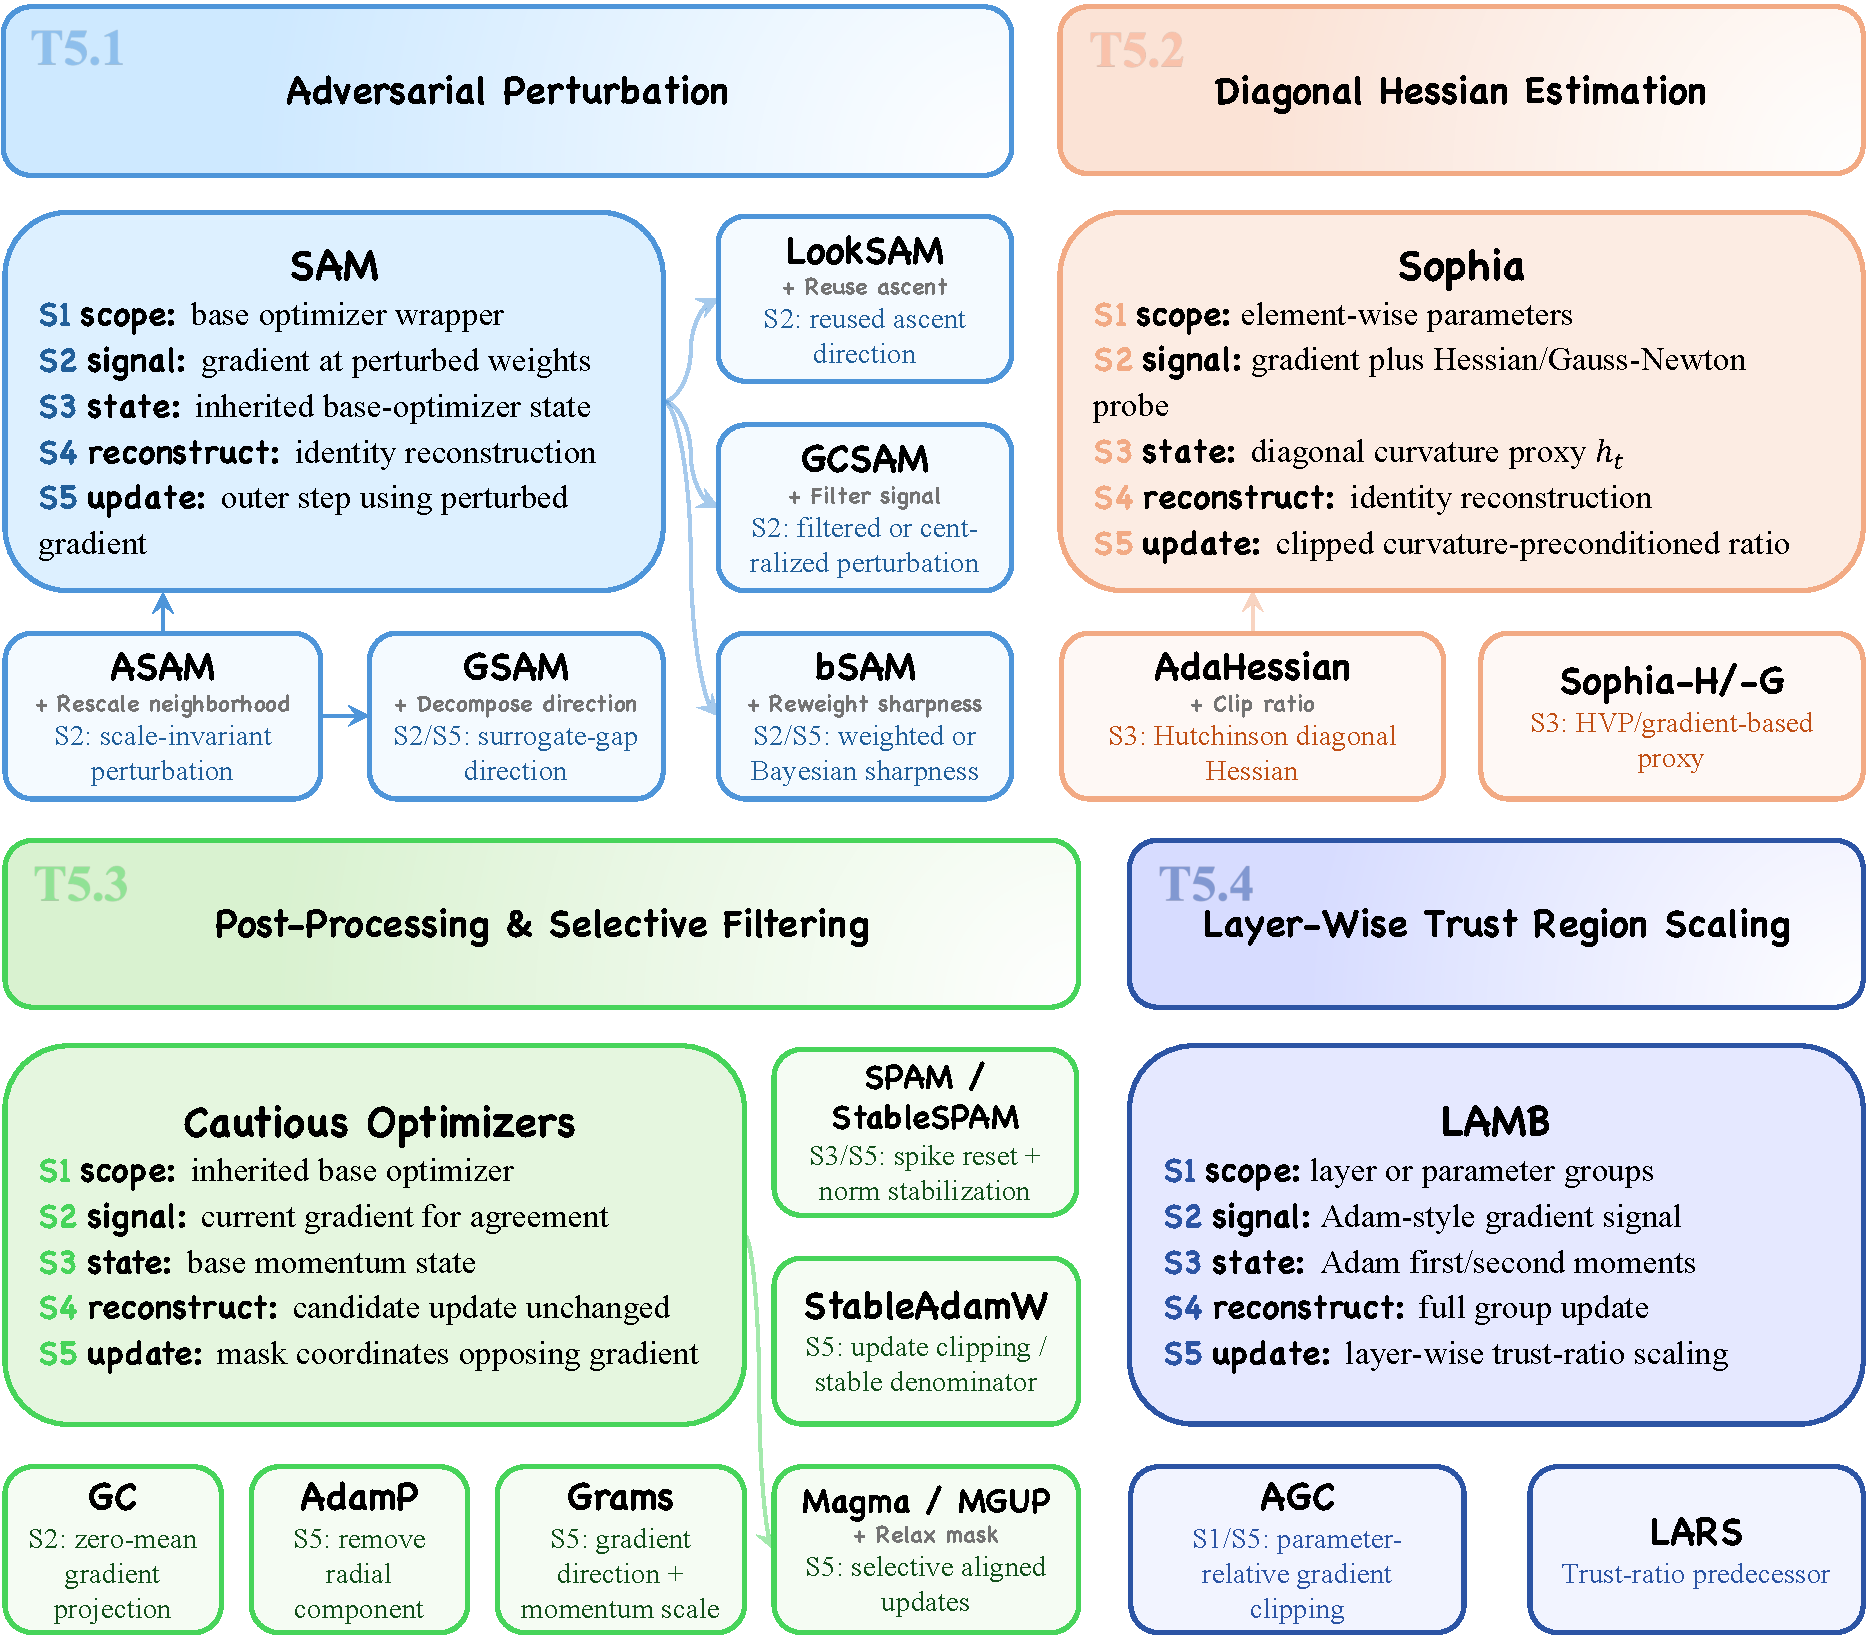
\includegraphics[width=0.75\linewidth]{figures/opt_t5.pdf}
  \caption{Mechanism schematic for T5 curvature-aware and geometric
  regularization methods.  The schematic organizes the family by where the
  geometric intervention enters the update: perturbed-gradient evaluation,
  diagonal-curvature estimation, post-update filtering, or layer-wise
  trust-region scaling.}
  \label{fig:t5_family_mechanism}
\end{figure}

% Auto-generated by code/generate_taxonomy_figures.py; do not edit by hand.
% \begin{table*}[!htbp]
%   \centering
%   \caption{Taxonomy of curvature-aware and geometry-regularized optimizers.}
%   \label{tab:t5_family_taxonomy}
%   \scriptsize
%   \setlength{\tabcolsep}{4pt}
%   \renewcommand{\arraystretch}{1.16}
%   \arrayrulecolor{optHiddenBlack}
%   \begin{tabularx}{\textwidth}{@{}>{\raggedright\arraybackslash}p{0.27\textwidth}>{\raggedright\arraybackslash}X@{}}
%     \hline
%     \textbf{Subclass} & \textbf{Optimizers} \\
%     \hline
%     \textbf{\textit{T5.1: Adversarial Perturbation (SAM Family)}} & SAM~\cite{foret2021sharpness}, ASAM~\cite{kwon2021asam}, GSAM~\cite{zhuang2022surrogate}, WSAM~\cite{yue2023sharpness}, bSAM~\cite{mollenhoff2022sam}, LookSAM~\cite{liu2022towards}, FriendlySAM~\cite{li2024friendly}, GCSAM~\cite{hassan2025gcsam} \\
%     \hline
%     \textbf{\textit{T5.2: Diagonal Hessian Estimation}} & Sophia~\cite{liu2023sophia}, AdaHessian~\cite{yao2021adahessian} \\
%     \hline
%     \textbf{\textit{T5.3: Update Post-Processing \& Selective Filtering}} & GC~\cite{yong2020gradient}, AdamP~\cite{heo2020adamp}, StableAdamW~\cite{wortsman2023stable}, Norm Loss~\cite{wortsman2023stable}, Stable WD~\cite{wortsman2023stable}, Grams~\cite{cao2024grams}, C-AdamW~\cite{liang2024cautious}, C-Lion~\cite{liang2024cautious}, SPAM~\cite{huang2025spam}, StableSPAM~\cite{huanggradientstabilizer}, Magma~\cite{joo2026surprising}, AlphaAdam~\cite{}, MGUP~\cite{chang2026mgup} \\
%     \hline
%     \textbf{\textit{T5.4: Layer-wise Trust Region Scaling}} & LAMB~\cite{you2019large}, AGC~\cite{brock2021high} \\
%     \hline
%   \end{tabularx}
% \end{table*}


\definecolor{hidden-blue}{HTML}{4a90e2}
\definecolor{hidden-black}{HTML}{333333}
\tikzstyle{my-box}=[
  rectangle,
  draw=hidden-black,
  rounded corners,
  text opacity=1,
  minimum height=1.5em,
  minimum width=5em,
  inner sep=2pt,
  align=center,
  fill opacity=.5,
]
\tikzstyle{root}=[
  align=center,
]
\tikzstyle{leaf}=[
  my-box,
  minimum height=1.5em,
  text=black,
  font=\normalsize,
  inner xsep=5pt,
  inner ysep=4pt,
  text width=10.5em,
  fill opacity=1,
]
\tikzstyle{leaf1}=[
  my-box,
  minimum height=1.5em,
  fill=yellow!32,
  text=black,
  font=\normalsize,
  inner xsep=5pt,
  inner ysep=4pt,
  text width=17em,
  align=left,
]
\tikzstyle{leaf2}=[
  my-box,
  minimum height=1.5em,
  fill=hidden-blue!57,
  text=black,
  font=\normalsize,
  inner xsep=5pt,
  inner ysep=4pt,
  text width=17em,
  align=left,
]
\tikzstyle{leaf3}=[
  my-box,
  minimum height=1.5em,
  fill=purple!27,
  text=black,
  font=\normalsize,
  inner xsep=5pt,
  inner ysep=4pt,
  text width=17em,
  align=left,
]
\tikzstyle{leaf4}=[
  my-box,
  minimum height=1.5em,
  fill=teal!30,
  text=black,
  font=\normalsize,
  inner xsep=5pt,
  inner ysep=4pt,
  text width=17em,
  align=left,
]

\begin{figure*}[!htbp]
\centering
\resizebox{\textwidth}{!}{
\begin{forest}
forked edges,
for tree={
grow=east,
reversed=true,
anchor=base west,
parent anchor=east,
child anchor=west,
base=left,
font=\large,
rectangle,
draw=hidden-black,
rounded corners,
align=left,
minimum width=4em,
edge+={darkgray, line width=1pt},
s sep=4pt,
inner xsep=5pt,
inner ysep=4pt,
line width=1.1pt,
ver/.style={rotate=90, child anchor=north, parent anchor=south, anchor=center},
},
where level=1{text width=11em, font=\normalsize}{},
where level=2{text width=34.5em, align=left, tier=citations, font=\small}{},
[
    T5-based Optimizers,
    ver, fill=brown!10!white, text=hidden-black, root
    [
        T5.1: Adversarial Perturbation \\ (SAM Family),
        fill=yellow!32, leaf1
        [{
            SAM~\cite{foret2021sharpness},
            ASAM~\cite{kwon2021asam},
            GSAM~\cite{zhuang2022surrogate},
            WSAM~\cite{yue2023sharpness},
            bSAM~\cite{mollenhoff2022sam},
            LookSAM~\cite{liu2022towards}, \\
            FriendlySAM~\cite{li2024friendly},
            GCSAM~\cite{hassan2025gcsam}
        }, fill=yellow!12]
    ]
    [
        T5.2: Diagonal Hessian Estimation,
        fill=hidden-blue!57, leaf2
        [{
            Sophia~\cite{liu2023sophia},
            AdaHessian~\cite{yao2021adahessian}
        }, fill=hidden-blue!15]
    ]
    [
        T5.3: Update Post-Processing \\ \& Selective Filtering,
        fill=purple!27, leaf3
        [{
            GC~\cite{yong2020gradient},
            AdamP~\cite{heo2020adamp},
            StableAdamW~\cite{wortsman2023stable},
            Norm Loss~\cite{wortsman2023stable},
            Stable WD~\cite{wortsman2023stable}, \\
            Grams~\cite{cao2024grams},
            C-AdamW~\cite{liang2024cautious},
            C-Lion~\cite{liang2024cautious},
            SPAM~\cite{huang2025spam},
            StableSPAM~\cite{huanggradientstabilizer},
            Magma~\cite{joo2026surprising}, \\
            MGUP~\cite{chang2026mgup}
        }, fill=purple!12]
    ]
    [
        T5.4: Layer-wise Trust Region Scaling,
        fill=teal!30, leaf4
        [{
            LAMB~\cite{you2019large},
            AGC~\cite{brock2021high}
        }, fill=teal!12]
    ]
  ]
\end{forest}
}
\caption{Taxonomy of curvature-aware and geometry-regularized optimizers.
The prefix C- denotes Cautious.}
\label{tab:t5_family_taxonomy}
\end{figure*}


\paragraph{Subclass structure.}
Figure~\ref{tab:t5_family_taxonomy} gives the complete optimizer membership for
T5.  The four subclasses below interpret that taxonomy figure by the dominant
geometric operation.
\begin{enumerate}[label=\textbf{T5.\arabic*},leftmargin=*,itemsep=2pt]
  \item \textbf{Adversarial perturbation (SAM family).}
  SAM replaces the ordinary gradient by a gradient measured at a local
  adversarial perturbation~\citep{foret2021sharpness}.  ASAM changes the
  perturbation geometry~\citep{kwon2021asam}.  Later variants modify the
  sharpness objective or its probabilistic interpretation
  ~\citep{zhuang2022surrogate,yue2023sharpness,mollenhoff2022sam}, reduce perturbation
  frequency~\citep{liu2022towards}, separate stochastic-noise components in
  the perturbation~\citep{li2024friendly}, or combine SAM with gradient
  centralization~\citep{hassan2025gcsam}.
  \item \textbf{Diagonal Hessian estimation.}
  Sophia maintains a diagonal Hessian or Gauss--Newton proxy and uses clipping
  to form an LLM-oriented trust-region-like update~\citep{liu2023sophia}.
  AdaHessian provides the earlier randomized diagonal-Hessian route
  ~\citep{yao2021adahessian}.
  \item \textbf{Update post-processing and selective filtering.}
  This subclass centralizes, projects, normalizes, masks, stabilizes, or
  selectively amplifies a gradient or candidate update after the base direction
  has been defined.  Gradient Centralization and AdamP are projection-style
  instances~\citep{yong2020gradient,heo2020adamp}, StableAdamW and its norm or
  decay components stabilize AdamW-style writeback~\citep{wortsman2023stable},
  Cautious Optimizers instantiate direction-consistency masks
  ~\citep{liang2024cautious}, Grams separates direction and adaptive
  magnitude~\citep{cao2024grams}, SPAM and StableSPAM target spike-aware or
  norm-stabilized writeback
  ~\citep{huang2025spam,huanggradientstabilizer}, Magma and
  MGUP occupy the selective-update and momentum-gradient-alignment corner of
  the subclass~\citep{joo2026surprising,chang2026mgup}.
  \item \textbf{Layer-wise trust-region scaling.}
  LAMB compares update and parameter norms to rescale Adam-style layer updates
  ~\citep{you2019large}, whereas AGC clips gradients relative to the receiving
  parameter group~\citep{brock2021high}.
\end{enumerate}

At the family level, a T5 method can be summarized as
\begin{align}
  \tilde{g}_t
  &=
  \mathcal{P}_t(g_t,\theta_t),\quad
  c_t =
  \mathcal{H}_t(\tilde{g}_t,\mathcal{S}_t), \\
  \Delta_t^{\mathrm{base}}
  &=
  \mathcal{U}_{\mathrm{base}}(\tilde{g}_t,\mathcal{S}_t,c_t),\quad
  \Delta_t =
  \mathcal{G}_t(\Delta_t^{\mathrm{base}},\tilde{g}_t,\theta_t,c_t), \\
  \theta_{t+1}
  &=
  \theta_t-\eta_t\Delta_t .
  \label{eq:t5-family-template}
\end{align}
Here $\mathcal{P}_t$ denotes the effective-gradient map, which is non-identity for SAM-style perturbations and some filtering methods, $c_t$ is an optional curvature or scale signal, $\mathcal{U}_{\mathrm{base}}$ is the underlying optimizer update, and $\mathcal{G}_t$ is the T5 geometry operator.  Ordinary AdamW with no wrapper is the identity case
$\mathcal{P}_t=I$, $\mathcal{H}_t=\varnothing$, and $\mathcal{G}_t=I$.

In the meta-pipeline, T5 primarily acts near S5, but different subclasses
enter through different interfaces.  T5.1 reaches S5 through an S0/S2
perturbed-gradient evaluation.  T5.2 modifies S3 by storing a curvature proxy
and modifies S5 by clipping the resulting ratio.  T5.3 uses S2 or S5 to filter
the gradient or candidate update.  T5.4 uses S1 to define layer or
parameter-group routes and S5 to apply group-level trust ratios.  S4 is
usually identity-like because the update remains full-dimensional unless the
method is primarily a T2 subspace method or a T4 state-compression method.

This definition fixes the boundary with the previous families.  A direct
AdamW variant remains T1 even if it improves stability, because its decisive
change is still the element-wise moment formula.  Muon, Shampoo, and GaLore
remain T2 because they change the matrix basis or subspace before the update
is formed.  Lion remains T3 because its sign map defines the base direction.
AdaFactor, 8-bit Adam, and Adam-mini remain T4 because they primarily alter
state representation.  By contrast, SAM can wrap SGD or AdamW, Cautious Lion
can wrap Lion, and LAMB can wrap an Adam-style update.  Their primary labels
come from the wrapper-level geometry added around the base optimizer.

\subsubsection{LMO-Driven Four-Axis Interpretation}
\label{sec:t5-lmo-four-axis}

T5 exposes the boundary between the LMO direction coordinate and the
post-direction geometry of an optimizer.  The LMO view explains how a base
direction is selected under a norm constraint.  T5 asks whether that direction
should be evaluated at a different point, clipped by curvature, filtered by
alignment, or rescaled by parameter-group geometry before it is written back.
In four-axis notation, the base optimizer first supplies
\begin{equation}
  \big((B_{\mathrm{a}},B_{\mathrm{u}}),\,
  \psi_{\mathrm{base}},\,\widehat{H}_t,\,
  \alpha,\,\widehat{g}_t,\,\mathcal{R}\big),
\end{equation}
and T5 appends an outer operator to the resulting step.  For methods whose
effective gradient is unchanged, Eq.~\eqref{eq:t5-family-template} reduces to
\begin{equation}
\begin{aligned}
  \Delta_t^{\mathrm{base}}
  = \mathcal{U}_{\mathrm{base}}(g_t,\mathcal{S}_t),
   \quad \Delta_t=\mathcal{G}_t\!\left(\Delta_t^{\mathrm{base}}, g_t, \theta_t\right), \quad
  \theta_{t+1}=\theta_t-\eta_t\Delta_t .
\end{aligned}
\label{eq:t5-geometry-wrapper}
\end{equation}
Here $\mathcal{U}_{\mathrm{base}}$ may be SGD, AdamW, Lion, Muon, or another
optimizer.  For most T5.3 and T5.4 methods, the base optimizer's four-axis
coordinates remain intact, and the T5 mechanism is the additional S5 map
$\mathcal{G}_t$.

SAM is different because it changes the point at which the gradient is
measured.  Its local objective can be written as
\begin{equation}
\begin{aligned}
  \min_{\theta}\ \max_{\|\epsilon\|\leq \rho}
  \mathcal{L}(\theta+\epsilon),
  \quad
  \epsilon_t
  \approx
  \rho\,\frac{g_t}{\|g_t\|_2}.
\end{aligned}
\label{eq:t5-sam-objective}
\end{equation}
The update then uses $\nabla \mathcal{L}(\theta_t+\epsilon_t)$ in place of the
ordinary mini-batch gradient.  This makes SAM an S0/S5 wrapper, where the inner
ascent direction is a local geometric probe, while the outer step can still
be executed by SGD, AdamW, or another base optimizer.  The price is the
second forward-backward pass needed to evaluate the perturbed gradient.

Diagonal-curvature methods fit more directly into Axes~II and~III.  Sophia-H
uses a stochastic Hessian-vector product to estimate a diagonal curvature
proxy, while Sophia-G uses a cheaper gradient-based proxy.  Both use clipping
to avoid unconstrained Newton-like steps~\citep{liu2023sophia}.  In schematic
form,
\begin{equation}
\begin{aligned}
  h_t=\beta_2 h_{t-1}+(1-\beta_2)\widehat{\operatorname{diag}}(H_t), \quad
  \Delta_t=\operatorname{clip}\!\left(\frac{m_t}{\gamma h_t+\epsilon}, -1, 1\right).
\end{aligned}
\label{eq:t5-sophia-clipping}
\end{equation}
AdaHessian is the earlier diagonal-Hessian route, using Hutchinson-style
estimation and Hessian-powered adaptive scaling~\citep{yao2021adahessian}.
Compared with AdamW, T5.2 therefore changes both the curvature estimator and
the final direction function.

Post-processing and layer-wise trust-region methods are simpler in the
four-axis view but important in practice.  A cautious filter can be expressed
as
\begin{equation}
  \mathcal{G}^{\mathrm{cautious}}(\Delta,g)
  =
  \Delta \odot \mathbf{1}[\Delta\odot g > 0],
\label{eq:t5-cautious-filter}
\end{equation}
up to the sign convention used for $\Delta$.  The key property is that only
coordinates whose proposed update agrees with the instantaneous gradient are
kept~\citep{liang2024cautious}.  A LAMB-style trust ratio instead rescales
the whole layer:
\begin{equation}
\begin{aligned}
  \Delta_t^{(l)}
  &=
  \phi_t^{(l)}\Delta_{t,\mathrm{Adam}}^{(l)},
  \quad
  \phi_t^{(l)}
  =
  \frac{\|\theta_t^{(l)}\|_2}
       {\|\Delta_{t,\mathrm{Adam}}^{(l)}\|_2+\epsilon}.
\end{aligned}
\label{eq:t5-lamb-ratio}
\end{equation}
Both operations illustrate the same principle, namely that T5 often leaves the base
direction geometry untouched, then constrains which parts of that direction
are written into the parameters and at what group-level scale.

\subsubsection{Representative Methods}
\label{sec:t5-methods}

\noindent
The following discussion follows the T5.1--T5.4 subclass order introduced
above.  Within each subclass, representative methods are grouped by the local
geometry operation they modify.

\paragraph{Adversarial Perturbation (SAM Family).}
\label{sec:t5-adversarial-perturbation}

The first branch changes the gradient evaluation point.  At the survey level,
SAM-style methods can be written as
\begin{equation}
\begin{aligned}
  \epsilon_t=\mathcal{A}_t(g_t,\theta_t;\rho), \quad
  \tilde{g}_t=\nabla_{\theta}\mathcal{L}(\theta_t+\epsilon_t), \quad
  \Delta_t=\mathcal{U}_{\mathrm{base}}(\tilde{g}_t,\mathcal{S}_t),
\end{aligned}
\label{eq:t5-adversarial-template}
\end{equation}
where $\mathcal{A}_t$ specifies the perturbation rule and
$\mathcal{U}_{\mathrm{base}}$ can be SGD, AdamW, or another first-order base
optimizer.
\begin{itemize}
  \setlength{\itemsep}{2pt}
  \item \textbf{Min--max anchor.}  SAM instantiates
  $\mathcal{A}_t$ by the approximate adversarial perturbation in
  Eq.~\eqref{eq:t5-sam-objective}, then updates with the perturbed gradient
  ~\citep{foret2021sharpness}.  This directly connects optimization to
  flatness-motivated generalization, but it also changes the cost model, because
  without approximation or reuse, one step requires two sequential
  forward-backward passes.
  \item \textbf{Perturbation geometry and sharpness objective.}  ASAM changes
  the neighborhood geometry to reduce sensitivity to parameter rescaling
  ~\citep{kwon2021asam}.  GSAM introduces a surrogate-gap objective and
  direction decomposition to balance loss decrease and sharpness reduction
  ~\citep{zhuang2022surrogate}.  WSAM treats weighted sharpness as a regularization
  term~\citep{yue2023sharpness}.  bSAM links the SAM objective to a Bayesian
  relaxation and motivates Adam-like uncertainty-aware variants
  ~\citep{mollenhoff2022sam}.
  \item \textbf{Perturbation frequency and signal composition.}  LookSAM
  targets the extra-gradient bottleneck by periodically refreshing or reusing
  the ascent direction~\citep{liu2022towards}.  FriendlySAM separates
  full-gradient and stochastic-gradient-noise components in the perturbation
  signal~\citep{li2024friendly}.  GCSAM combines the perturbation route
  with gradient centralization before the ascent step
  ~\citep{hassan2025gcsam}.
\end{itemize}

The common thread is perturbed-gradient evaluation.  Claims about this branch should therefore be read through the
matched-compute lens: improvements under a fixed number of tokens do not
automatically imply improvements under a fixed wall-clock or accelerator
budget.

\paragraph{Diagonal Hessian Estimation.}
\label{sec:t5-diagonal-hessian}

The second branch replaces AdamW's squared-gradient denominator with a more
explicit diagonal curvature proxy.  A compact template is
\begin{align}
  q_t
  &\approx
  \widehat{\operatorname{diag}}(H_t)
  \quad\text{or}\quad
  \widehat{\operatorname{diag}}(G_t^{\mathrm{GN}}),\\
  h_t
  &=
  \beta_2 h_{t-1}+(1-\beta_2)q_t,\quad
  \Delta_t =
  \Pi_{\gamma}\!\left(\frac{m_t}{h_t+\epsilon}\right),
  \label{eq:t5-diagonal-curvature-template}
\end{align}
where $\Pi_{\gamma}$ denotes a clipping or trust-region map that prevents
small or noisy curvature estimates from producing unbounded Newton-like
coordinates.
\begin{itemize}
  \setlength{\itemsep}{2pt}
  \item \textbf{LLM-oriented clipped curvature.}  Sophia is the main
  representative method for LLM pretraining.  Sophia-H estimates curvature
  with a stochastic Hessian-vector product, whereas Sophia-G uses a cheaper
  gradient-based proxy.  Both combine the proxy with a clipped coordinate-wise
  update~\citep{liu2023sophia}.
  \item \textbf{Diagonal-Hessian predecessor.}  AdaHessian uses randomized
  Hessian-vector products to estimate diagonal curvature and smooths that
  estimate before applying Hessian-powered adaptive scaling
  ~\citep{yao2021adahessian}.  It establishes the diagonal-Hessian route, but
  its target regime predates current LLM pretraining protocols.
\end{itemize}

T5.2 is adjacent to both T1 and T2 but distinct from each.  It differs from T1
because its denominator is intended to approximate Hessian or Gauss--Newton
curvature.  It differs from T2 because it
remains diagonal.  Benchmark reports should therefore expose Hessian-estimation
cadence, HVP batch, Sophia-H versus Sophia-G choice, clipping parameters, and
mixed-precision behavior.

\paragraph{Update Post-Processing and Selective Filtering.}
\label{sec:t5-post-processing}

The third branch acts after a base direction has been formed.  The taxonomy
figure lists methods whose surface forms differ substantially, but the common
mechanism is an additional operator between the base optimizer and parameter
writeback.  At this level, the branch can be summarized as
\begin{equation}
\begin{aligned}
  \bar{\Delta}_t=\Pi_t(\Delta_t^{\mathrm{base}},g_t,\theta_t),\quad
  M_t=\mathcal{M}_t(\bar{\Delta}_t,g_t,\theta_t,\mathcal{S}_t),\quad
  \Delta_t=M_t\odot\bar{\Delta}_t ,
\end{aligned}
\label{eq:t5-filter-template}
\end{equation}
where $\Pi_t$ may centralize, project, normalize, or stabilize the candidate
update, and $M_t$ is a coordinate mask or selection weight.  The all-ones mask
recovers projection-only methods.  This template deliberately separates
post-processing from base-direction construction, because $\Delta_t^{\mathrm{base}}$
may come from AdamW, Lion, Muon, or another optimizer, while the T5.3
contribution is the subsequent geometric test, projection, norm control, or
selection policy.
\begin{itemize}
  \setlength{\itemsep}{2pt}
  \item \textbf{Projection and radial control.}  Gradient Centralization
  subtracts the mean from gradient vectors or convolutional kernels, placing
  the update in a zero-mean subspace that can be attached to SGD, Adam, or
  related optimizers~\citep{yong2020gradient}.  AdamP addresses a different
  geometric failure mode by removing radial components for
  scale-invariant weights, so that accumulated momentum does not mainly increase parameter
  norms~\citep{heo2020adamp}.  Both methods leave the base optimizer
  recognizable, and their contribution is the projection $\Pi_t$ before writeback.
  \item \textbf{Stabilized writeback and norm control.}  StableAdamW analyzes
  loss spikes caused by unstable AdamW-style update magnitudes and motivates
  stabilized denominators or AdamW--AdaFactor hybrids~\citep{wortsman2023stable}.
  The Norm Loss and Stable WD entries in Figure~\ref{tab:t5_family_taxonomy}
  should be read as related S5 regularization components from the same
  stability-oriented design space.  Their
  role in this taxonomy is to expose norm and decay control as writeback
  mechanisms that can change stability without changing the moment estimator.
  \item \textbf{Direction consistency and magnitude separation.}  Cautious
  Optimizers apply the mask in Eq.~\eqref{eq:t5-cautious-filter} to a proposed
  update, keeping coordinates only when the update and instantaneous gradient
  agree under the paper's sign convention~\citep{liang2024cautious}.  This is
  why Cautious AdamW (C-AdamW) and Cautious Lion (C-Lion) share the same T5.3
  label even though their base directions belong to T1 and T3, respectively.  Grams makes a complementary
  separation, where the current gradient supplies direction, while momentum mainly
  supplies adaptive magnitude scaling~\citep{cao2024grams}.
  \item \textbf{Spike-aware and selective-update policies.}  SPAM identifies
  gradient spikes in LLM training as a stability bottleneck and combines
  spike-aware clipping, momentum reset, and sparse momentum behavior
  ~\citep{huang2025spam}.  StableSPAM broadens this idea into norm-stabilized
  writeback, keeping the instantaneous gradient direction while replacing
  unstable update magnitudes with running norm statistics
  ~\citep{huanggradientstabilizer}.  Magma demonstrates that random or
  momentum-aligned masks can be effective when applied to adaptive optimizer
  updates~\citep{joo2026surprising}, whereas MGUP assigns larger steps to
  momentum-gradient-aligned coordinates and smaller nonzero steps elsewhere
  ~\citep{chang2026mgup}.
\end{itemize}

The common thread is that T5.3 filters operate on gradients or candidate
updates after the base optimizer's core direction has been selected.  This
also fixes the boundary with T3.  Sign methods define the base direction
itself, whereas T5.3 methods accept, reject, rescale, or regularize an already
computed direction.  Consequently, a Lion wrapper with a cautious mask belongs
to T5.3 as a wrapper-level contribution, while Lion itself remains T3.

\paragraph{Layer-Wise Trust-Region Scaling.}
\label{sec:t5-layerwise-trust-region}

The fourth branch uses parameter-group geometry to determine the step scale.
For a layer or parameter group $l$, the representative form is
\begin{align}
  r_t^{(l)}
  &=
  \frac{\|\theta_t^{(l)}\|_2}
       {\|\Delta_{t,\mathrm{base}}^{(l)}\|_2+\epsilon},\quad
  \Delta_t^{(l)}
  =
  \Psi(r_t^{(l)})\,\Delta_{t,\mathrm{base}}^{(l)}, \\
  g_t^{(l)}
  &\leftarrow
  g_t^{(l)}
  \min\!\left(
  1,\frac{\tau\|\theta_t^{(l)}\|_2}{\|g_t^{(l)}\|_2+\epsilon}
  \right),
  \label{eq:t5-layerwise-template}
\end{align}
where the first line is a trust-ratio update and the second line is an
adaptive clipping rule.
\begin{itemize}
  \setlength{\itemsep}{2pt}
  \item \textbf{Trust-ratio update.}  LAMB first forms an Adam-style update and
  then rescales it by the layer-wise ratio in Eq.~\eqref{eq:t5-lamb-ratio}
  ~\citep{you2019large}.  Its contribution is
  the S1/S5 layer-wise grouping and trust-ratio writeback used for large-batch
  training.
  \item \textbf{Parameter-relative clipping.}  Adaptive Gradient Clipping
  clips a layer or unit when the gradient norm is too large relative to the
  parameter norm~\citep{brock2021high}.  Unlike fixed global clipping, the
  threshold scales with the receiving parameter group.
\end{itemize}

Layer-wise trust-region methods are syntactically easy to combine with
Adam-style bases, but their behavior depends on parameter-group conventions.
Benchmarks should state which tensors are excluded, how zero or near-zero
norms are handled, whether trust ratios are clipped, and whether the ratio is
applied before or after weight decay and global clipping.

\subsubsection{Effect-Target Assessment}
\label{sec:t5-effect-assessment}

T5 acts on the geometry of the candidate step rather than on the base
optimizer alone.  The expected benefit is therefore stability or
generalization: SAM-style perturbations seek flatter neighborhoods, diagonal
curvature methods clip steps by local curvature, post-update filters suppress
harmful components, and layer-wise trust ratios control scale mismatch across
parameter groups.  Each mechanism also adds a protocol-dependent cost.  SAM
spends extra forward-backward work~\citep{foret2021sharpness}; Sophia-style
updates rely on curvature proxies and clipping choices~\citep{liu2023sophia};
LAMB-style trust ratios depend on layer norms and excluded tensors
~\citep{you2019large}.  Table~\ref{tab:t5_effect_assessment} summarizes the
mechanism-derived performance priors.

\begin{table*}[b]
  \centering
  \caption{Mechanism-informed effect assessment for T5 subclasses.  The
  entries are design priors for benchmark planning, not empirical
  conclusions.}
  \label{tab:t5_effect_assessment}
  \scriptsize
  \setlength{\tabcolsep}{3pt}
  \renewcommand{\arraystretch}{1.08}
  \begin{tabularx}{\textwidth}{@{}Y Y Y@{}}
    \toprule
    Primary target & Likely cost or failure mode & Benchmark focus \\
    \midrule
    \rowcolor{famT5!18}\multicolumn{3}{c}{\textbf{\textcolor{famT5!62!black}{T5: Curvature-aware and geometric regularization}}} \\
    \rowcolor{famT5!8}\multicolumn{3}{@{}l@{}}{\textbf{\textcolor{famT5!62!black}{T5.1 Adversarial perturbation (SAM family)}}} \\
      O6 generalization, O4 flatness
      & Extra forward-backward pass, radius sensitivity, wall-clock loss
      & Matched-token vs.\ matched-compute curves, radius and frequency, downstream evaluation \\
    \rowcolor{famT5!8}\multicolumn{3}{@{}l@{}}{\textbf{\textcolor{famT5!62!black}{T5.2 Diagonal Hessian estimation}}} \\
      O1 convergence, O4 stability via clipped curvature
      & HVP overhead, clipping sensitivity, stale curvature
      & Estimation cadence, Sophia-H vs.\ Sophia-G, clipping rule \\
    \rowcolor{famT5!8}\multicolumn{3}{@{}l@{}}{\textbf{\textcolor{famT5!62!black}{T5.3 Update post-processing and selective filtering}}} \\
      O4 stability, O5 tuning width
      & May drop useful descent components, extra hyperparameters
      & Same base with/without filter, kept-coordinate ratio, spike rate \\
    \rowcolor{famT5!8}\multicolumn{3}{@{}l@{}}{\textbf{\textcolor{famT5!62!black}{T5.4 Layer-wise trust-region scaling}}} \\
      O4/O5 under large batch and heterogeneous layers
      & Trust-ratio instability at small norms, exclusion sensitivity
      & Layer-wise norms, excluded tensors, clipping order, large-batch scaling \\
    \bottomrule
  \end{tabularx}
\end{table*}


The distinction between mechanism and observed effect is especially important
for this family.  A method belongs to T5 because it imposes a geometric
constraint; it need not improve generalization in every benchmark.  Conversely,
a T1 or T2 optimizer can be stable without becoming T5.  Budgeted optimizer
studies such as Schlotthauer et al.~\citep{schlotthauer2025budget} make this
point concrete: extra computation can change the apparent ranking if the
comparison is made at fixed steps rather than fixed compute.  The benchmark
summary in Sec.~\ref{sec:benchmark-family-summary} is consistent with this
caution: T5 methods are competitive in limited regimes, but they do not show a
uniform advantage under the current LLM benchmark.